\documentclass{article}

%% Packages %%

\usepackage{layout}
\usepackage{xcolor}
\usepackage{amsfonts}
\usepackage{hyperref}
\usepackage{setspace}
\hypersetup{
    colorlinks=true,
    linkcolor=black,
    filecolor=black!5,
    urlcolor=black,
    pdftitle={Vernon Grant},
    pdfpagemode=FullScreen,
}
\usepackage[a4paper,top=1cm,bottom=1cm,left=1.5cm,right=1.5cm]{geometry}


%% Document Margins %%

\marginparwidth 0pt
\marginparsep 0pt

%% Show the frames so we can make adjustments to margins.
%% \usepackage{showframe}

%% Tikz %%

\usepackage{tikz}
\usetikzlibrary{patterns}
\usetikzlibrary {arrows.meta}

%% Global Variables %%

\newcommand{\DiagramMaxWidth}{18cm}

\newcommand{\ExternalLink}{%
    \tikz[x=1.2ex, y=1.2ex, baseline=-0.05ex]{%
        \begin{scope}[x=1ex, y=1ex]
            \clip (-0.1,-0.1)
                --++ (-0, 1.2)
                --++ (0.6, 0)
                --++ (0, -0.6)
                --++ (0.6, 0)
                --++ (0, -1);
            \path[draw,
                line width = 0.5,
                rounded corners=0.5]
                (0,0) rectangle (1,1);
        \end{scope}
        \path[draw, line width = 0.5] (0.5, 0.5)
            -- (1, 1);
        \path[draw, line width = 0.5] (0.6, 1)
            -- (1, 1) -- (1, 0.6);
        }
    }

% Document:
\begin{document}

%% ------------------- %%
%% Introduction Header %%
%% ------------------- %%

\noindent
\begin{tikzpicture}[fill=white]
  %% Outer rectangle
  \draw[anchor=north west, color=black] (0,0) rectangle (18,3);

  %% Profile photo
  \node[inner sep=0pt, anchor=north west] (Vernon Grant) at (0,3)
       {
\includegraphics[width=2.9855cm]{profile.jpg}};
  \draw (3.43,2.4) node[anchor=north west] (a) {\Huge Vernon Grant};
  \draw (4.35,1.35) node[text=black!50, anchor=north west] (b) {\Large {\emph {Web Developer}}};

  %% Social media
  \draw[fill=white] (9,3) rectangle (13,2) node[pos=.5] {\href{http://example.com}{\ExternalLink GitHub}};
  \draw[fill=white] (9,2) rectangle (13,1) node[pos=.5] {\href{http://example.com}{\ExternalLink Twitter}};
  \draw[fill=white] (9,1) rectangle (13,0) node[pos=.5] {\href{http://example.com}{\ExternalLink LinkedIn}};

  %% Contact details
  \draw (13,3) rectangle (18,2) node[pos=.5] {vernon@ruppell.io};
  \draw (13,2) rectangle (18,1) node[pos=.5] {+270 0000 0000};
  \draw (13,1) rectangle (18,0) node[pos=.5] {Cape Town, South Africa};
\end{tikzpicture}
\break

%% ----------------- %%
%% Summary Statement %%
%% ----------------- %%

\noindent

\begin{tikzpicture}[fill=white]
  \draw (0,0) rectangle (9,1) node at (4.5,.5) {\large Summary Statement};
  \draw[color=black] (9,0.5) -- (18,0.5);
\end{tikzpicture}

\vspace{0.5cm}
\noindent I am an South African Web Developer with over five years of experience working in Hong Kong. I have developed expertise across various programming languages such as PHP, JavaScript, C, Clojure and more. I'm a very fast learner and enjoy coming up with simple and maintainable solutions to problems. While also having a keen eye for business analysis and problem-solving abilities that make me an asset to any company or organization looking to expand their digital footprint.
\vspace{0.65cm}

%% ---------- %%
%% Experience %%
%% ---------- %%

\noindent

\begin{tikzpicture}[fill=white]
  \draw (0,0) rectangle (9,1) node at (4.5,.5) {\large Professional Experience};
  \draw[color=black] (9,0.5) -- (18,0.5);
\end{tikzpicture}

% Full-Stack Web Developer
\vspace{0.5cm}

\begin{doublespace}
  \noindent {\Large Full-Stack Web Developer} \newline
  \noindent {\large \href{http://example.com}{\ExternalLink Ruppell Limited} | 2018 - Current \hfill \emph{Hong Kong}}
\end{doublespace}
\noindent I was responsible for developing both frontend (client-side scripting) as well as backend (server-side programming) solutions. I had to make use of various frameworks and languages such as Electron, Flutter, Bash, C, JavaScript, PHP, Clojure and more. I also managed virtual servers by updating SSL certificates, extracting statistical data from databases and keeping general security and backups up to date.

% Web Developer
\vspace{0.5cm}
\begin{doublespace}
  \noindent {\Large Web Developer} \newline
  \noindent {\large \href{http://example.com}{\ExternalLink Trinity International Limited}  | 2015 - 2018 \hfill \emph{Hong Kong}}
\end{doublespace}
\noindent I was responsible for creating and maintaining websites by using various programming languages such as HTML, CSS, JavaScript and PHP. I was expected to design user-friendly interfaces that can be easily navigated through on mobile, tablet and desktop devices. Apart from this I had to make use of SEO (Search Engine Optimization) techniques to help improve the visibility and ranking of the companies websites online.
\vspace{0.5cm}

% General Office Administrator
\begin{doublespace}
  \noindent {\Large General Office Administrator} \newline
  \noindent {\large \href{http://example.com}{\ExternalLink Seedland International Limited} | 2010 - 2015 \hfill \emph{Hong Kong}}
\end{doublespace}
\noindent As general office administrator, I was responsible for managing and coordinating various administrative tasks within the company, such as answering phones, greeting visitors, handling mail, scheduling appointments, maintaining filing systems, organizing meetings, arranging travel plans, preparing reports, processing expense claims, overseeing office supplies and inventory management.

\vspace{0.65cm}

%% ---------------- %%
%% Higher Education %%
%% ---------------- %%

\noindent

\begin{tikzpicture}[fill=white]
  \draw (0,0) rectangle (9,1) node at (4.5,.5) {\large Higher Education};
  \draw[color=black] (9,0.5) -- (18,0.5);
\end{tikzpicture}
\break

\noindent Lorem ipsum dolor sit amet, consectetur adipiscing elit, sed do eiusmod tempor incididunt ut labore et dolore magna aliqua. Ut enim ad minim veniam, quis nostrud exercitation ullamco laboris nisi ut aliquip ex ea commodo consequat. Duis aute irure dolor in reprehenderit in voluptate velit esse cillum dolore eu fugiat nulla pariatur. Excepteur sint occaecat cupidatat non proident, sunt in culpa qui officia deserunt mollit anim id est laborum.
\break
\break

%% --------------- %%
%% Recent Projects %%
%% --------------- %%

\noindent

\begin{tikzpicture}[fill=white]
  \draw (0,0) rectangle (9,1) node at (4.5,.5) {\large Recent Projects};
  \draw[color=black] (9,0.5) -- (18,0.5);
\end{tikzpicture}
\break

\noindent Lorem ipsum dolor sit amet, consectetur adipiscing elit, sed do eiusmod tempor incididunt ut labore et dolore magna aliqua. Ut enim ad minim veniam, quis nostrud exercitation ullamco laboris nisi ut aliquip ex ea commodo consequat. Duis aute irure dolor in reprehenderit in voluptate velit esse cillum dolore eu fugiat nulla pariatur. Excepteur sint occaecat cupidatat non proident, sunt in culpa qui officia deserunt mollit anim id est laborum.
\break
\break


%% They are responsible for designing user interfaces that allow users to interact with their content in an intuitive way. Additionally, they may be tasked with creating databases, managing server configurations, optimizing site performance, and ensuring security measures comply with industry standards.

%% A WordPress Developer is someone who has expertise in developing websites using the open-source content management system (CMS) called "Wordpress". They are responsible for creating and maintaining sites that use this CMS, which includes themes or templates to customize a site's look & feel as well as plugins/extensions to add functionality. WordPress Developers must have strong coding skills in PHP, HTML5, CSS3, JavaScript (jQuery), MySQL database management system, etc., and be familiar with the latest versions of these technologies for optimum performance on websites they develop or maintain.


\pagebreak

\section{Pre-Algebra}
\subsection{The types of numbers}
\vspace{\fill}
\resizebox{\DiagramMaxWidth}{!}{
    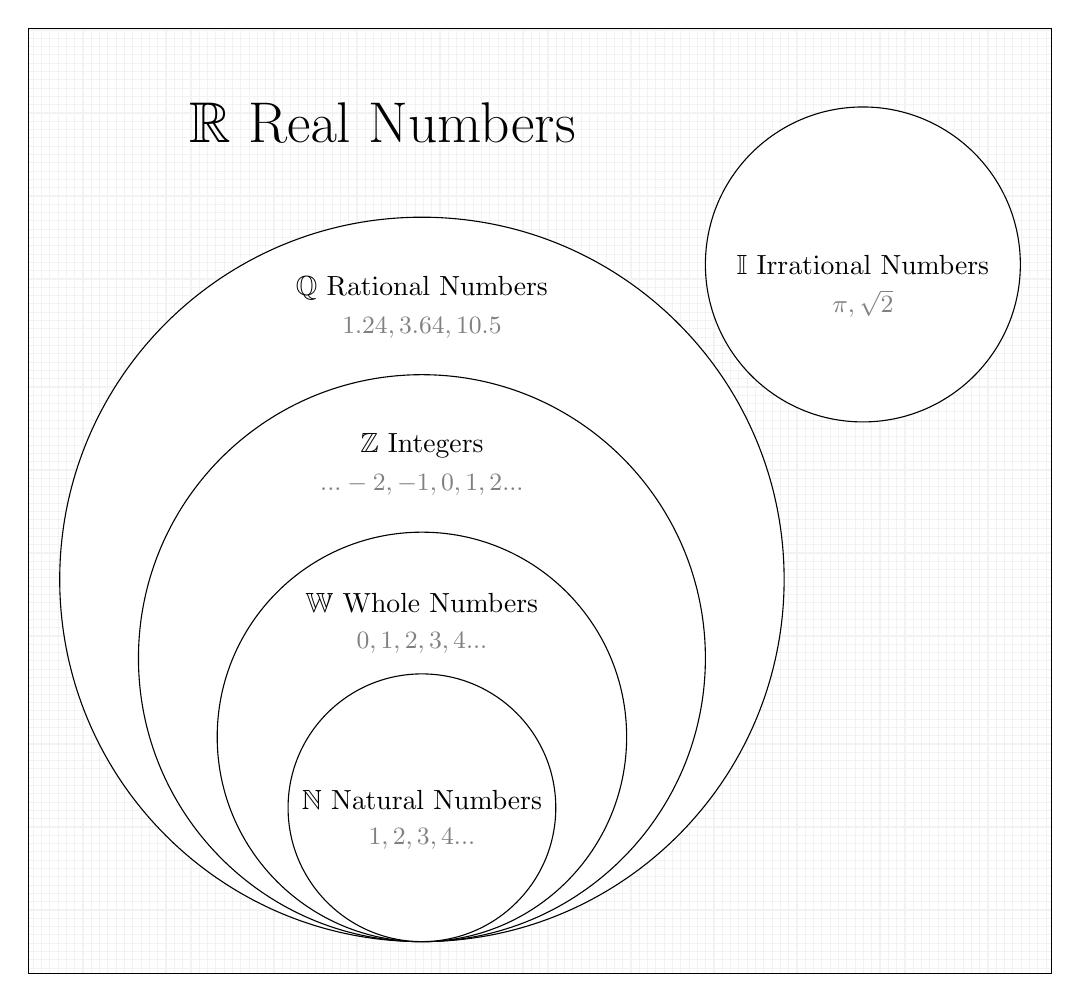
\begin{tikzpicture}[fill=white]
        % Real numbers
        \draw[pattern=grid, pattern color=black!5] (-7,-6) rectangle (6,6)
        (-2.5, 4.8) node {\huge{$\mathbb{R}$ Real Numbers}};

        % Irrational numbers
        \draw[black, fill=white] (3.6, 3) circle (2cm)
        (3.6, 3) node {$\mathbb{I}$ Irrational Numbers}
        (3.6, 2.5) node[color=gray] {\small{$\pi, \sqrt{2}$}};

        % Rational numbers
        \draw[black, fill=white] (-2,-1) circle (4.6cm)
        (-2,2.7) node {$\mathbb{Q}$ Rational Numbers}
        (-2,2.2) node[color=gray] {\small{$1.24, 3.64, 10.5$}};

        % Integer numbers
        \draw[black, fill=white] (-2,-2) circle (3.6cm)
        (-2, 0.7) node {$\mathbb{Z}$ Integers}
        (-2, 0.2) node[color=gray] {\small{$...-2, -1, 0, 1, 2 ...$}};

        % Whole numbers
        \draw[black, fill=white] (-2,-3) circle (2.6cm)
        (-2,-1.3) node {$\mathbb{W}$ Whole Numbers}
        (-2,-1.8) node[color=gray] {\small{$0, 1, 2, 3, 4 ...$}};

        % Natural numbers
        \draw[black, fill=white] (-2,-3.9) circle (1.7cm)
        (-2,-3.8) node {$\mathbb{N}$ Natural Numbers}
        (-2,-4.3) node[color=gray] {\small{$1, 2, 3, 4 ...$}};
    \end{tikzpicture}
}
\vspace{\fill}
\pagebreak

\subsection{Order of Operations}
\vspace{\fill}
\resizebox{\DiagramMaxWidth}{!}{
    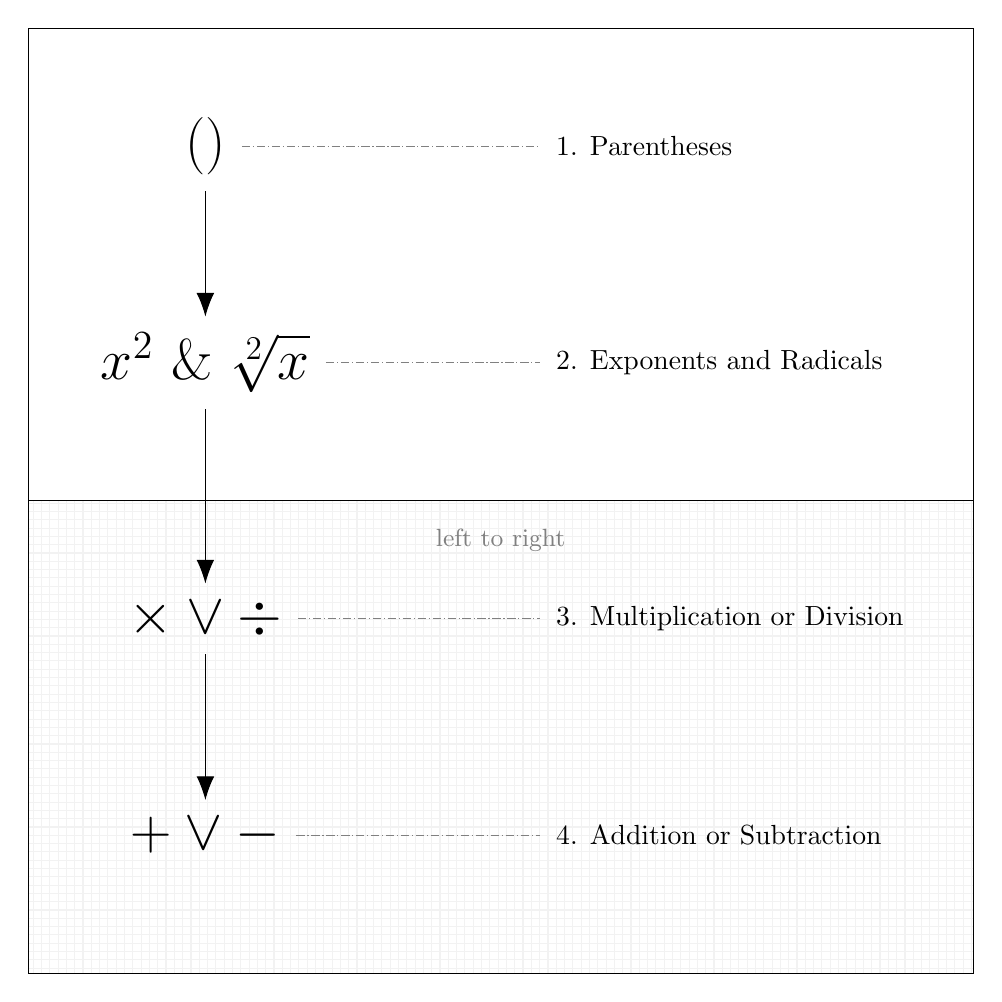
\begin{tikzpicture}[fill=white]
        \draw (0,0) rectangle (12,12);
        \draw[pattern=grid, pattern color=black!5] (0,0) rectangle (12,6);
        \draw[line width=5pt]
            % Parentheses
            (2.25,10.5) node[fill=white] (p) {\huge{$()$}}
            (6.5,10.5) node[anchor=west] (pp) {1. Parentheses}

            % Exponents
            (2.25,7.75) node[fill=white] (e) {\huge{$x^2$ \& $\sqrt[2]{x}$}}
            (6.5,7.75) node[anchor=west] (ee) {2. Exponents and Radicals}
            (6, 5.5) node[color=gray, anchor=center] {\small{left to right}}

            % Multiplication and division
            (2.25,4.5) node (m) {\huge{$\times \lor \div$}}
            (6.5,4.5) node[anchor=west] (mm) {3. Multiplication or Division}

            % Addition and Subtraction
            (2.25,1.75) node (a) {\huge{$+ \lor -$}}
            (6.5,1.75) node[anchor=west] (aa) {4. Addition or Subtraction};

        \draw[-{Latex[length=3mm]}] (p) -- (e);
        \draw[-{Latex[length=3mm]}] (e) -- (m);
        \draw[-{Latex[length=3mm]}] (m) -- (a);

        \draw[densely dash dot,color=gray] (p) -- (pp);
        \draw[densely dash dot,color=gray] (e) -- (ee);
        \draw[densely dash dot,color=gray] (m) -- (mm);
        \draw[densely dash dot,color=gray] (a) -- (aa);
    \end{tikzpicture}
}
\vspace{\fill}
\pagebreak

\subsection{Addition and Subtraction}
\subsection{Multiplication and Division}
\subsection{Fractions}
\pagebreak

\subsection{Least common multiple (LCM)}
\vspace{\fill}
\resizebox{\DiagramMaxWidth}{!}{
    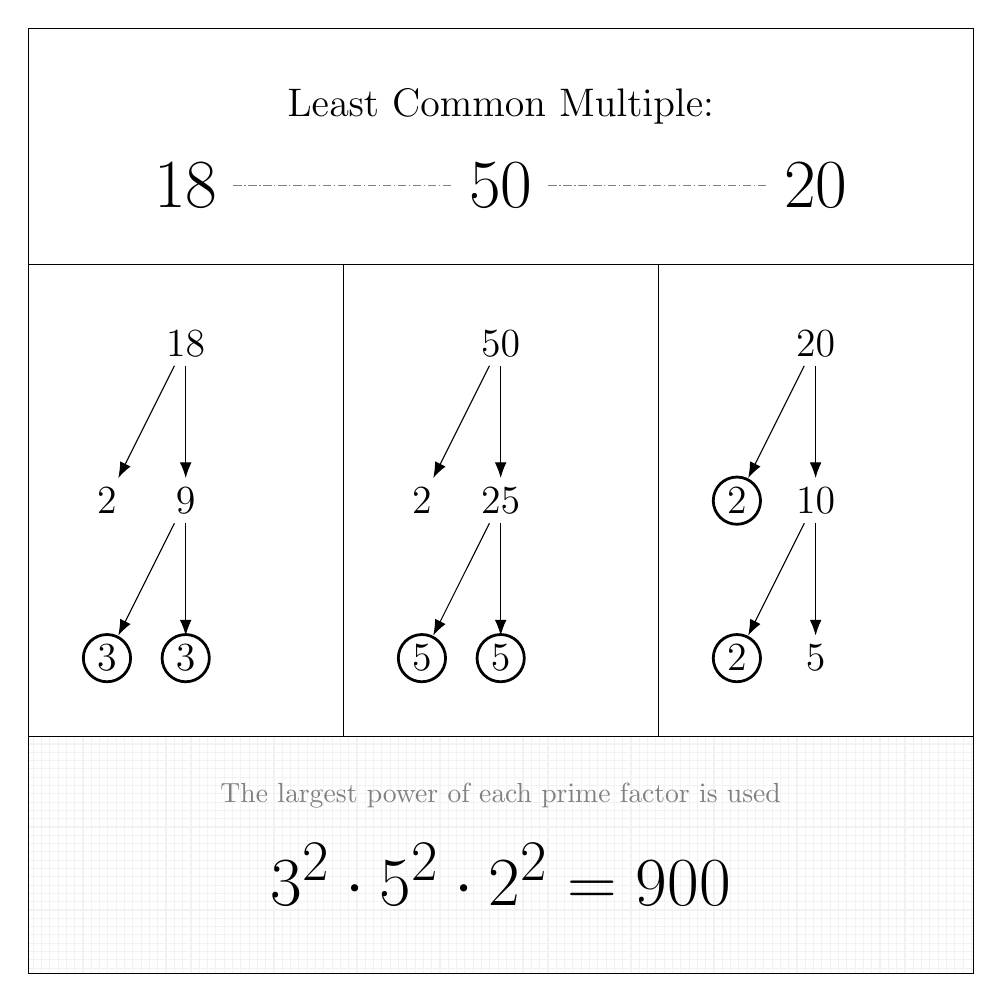
\begin{tikzpicture}[fill=white]
        \draw (0,0) rectangle (12,12);
        % Least common multiple
        \draw[line width=5pt]
            (6,11) node[anchor=center] {\Large Least Common Multiple:}
            (2,10) node[anchor=center] (a) {\Huge $18$}
            (6,10) node[anchor=center] (b) {\Huge $50$}
            (10,10) node[anchor=center] (c) {\Huge $20$};

        % Grid guidelines.
        \draw[-, ystep=9, xstep=4] (0,3) grid (12,9);

        % Factorizations.
        \draw (2,8) node[fill=white, anchor=center] (a1) {\Large $18$};
        \draw (1,6) node[fill=white, anchor=center] (a2) {\Large $2$};
        \draw (2,6) node[fill=white, anchor=center] (a3) {\Large $9$};
        \draw (1,4) node[fill=white, anchor=center] (a4) {\Large $3$};
        \draw (2,4) node[fill=white, anchor=center] (a5) {\Large $3$};
        \draw[-{Latex[length=2mm]}] (a1) -- (a2);
        \draw[-{Latex[length=2mm]}] (a1) -- (a3);
        \draw[-{Latex[length=2mm]}] (a3) -- (a4);
        \draw[-{Latex[length=2mm]}] (a3) -- (a5);

        \draw (6,8) node[fill=white, anchor=center] (b1) {\Large $50$};
        \draw (5,6) node[fill=white, anchor=center] (b2) {\Large $2$};
        \draw (6,6) node[fill=white, anchor=center] (b3) {\Large $25$};
        \draw (5,4) node[fill=white, anchor=center] (b4) {\Large $5$};
        \draw (6,4) node[fill=white, anchor=center] (b5) {\Large $5$};
        \draw[-{Latex[length=2mm]}] (b1) -- (b2);
        \draw[-{Latex[length=2mm]}] (b1) -- (b3);
        \draw[-{Latex[length=2mm]}] (b3) -- (b4);
        \draw[-{Latex[length=2mm]}] (b3) -- (b5);

        \draw (10,8) node[fill=white, anchor=center] (c1) {\Large $20$};
        \draw (9,6) node[fill=white, anchor=center] (c2) {\Large $2$};
        \draw (10,6) node[fill=white, anchor=center] (c3) {\Large $10$};
        \draw (9,4) node[fill=white, anchor=center] (c4) {\Large $2$};
        \draw (10,4) node[fill=white, anchor=center] (c5) {\Large $5$};
        \draw[-{Latex[length=2mm]}] (c1) -- (c2);
        \draw[-{Latex[length=2mm]}] (c1) -- (c3);
        \draw[-{Latex[length=2mm]}] (c3) -- (c4);
        \draw[-{Latex[length=2mm]}] (c3) -- (c5);

        \draw[line width=1pt] (9,6) circle (0.3);
        \draw[line width=1pt] (9,4) circle (0.3);
        \draw[line width=1pt] (6,4) circle (0.3);
        \draw[line width=1pt] (5,4) circle (0.3);
        \draw[line width=1pt] (1,4) circle (0.3);
        \draw[line width=1pt] (2,4) circle (0.3);

        % Solution
        \draw[pattern=grid, pattern color=black!5] (0,0) rectangle (12,3)
            (6,1.25) node[anchor=center] {\Huge $3^2 \cdot 5^2 \cdot 2^2 = 900$}
            (6,2.25) node[anchor=center, color=gray] {The largest power of each prime factor is used};

        \draw[densely dash dot,color=gray] (a) -- (b);
        \draw[densely dash dot,color=gray] (b) -- (c);
    \end{tikzpicture}
}
\vspace{\fill}
\pagebreak

\subsection{Greatest common divisor (GCD)}
\vspace{\fill}
\begin{tikzpicture}[fill=white]
    \draw (0,0) rectangle (12,12);
        % Least common multiple
\end{tikzpicture}
\vspace{\fill}
\pagebreak

\subsection{Laws of exponents}
\vspace{\fill}
\resizebox{\DiagramMaxWidth}{!}{
    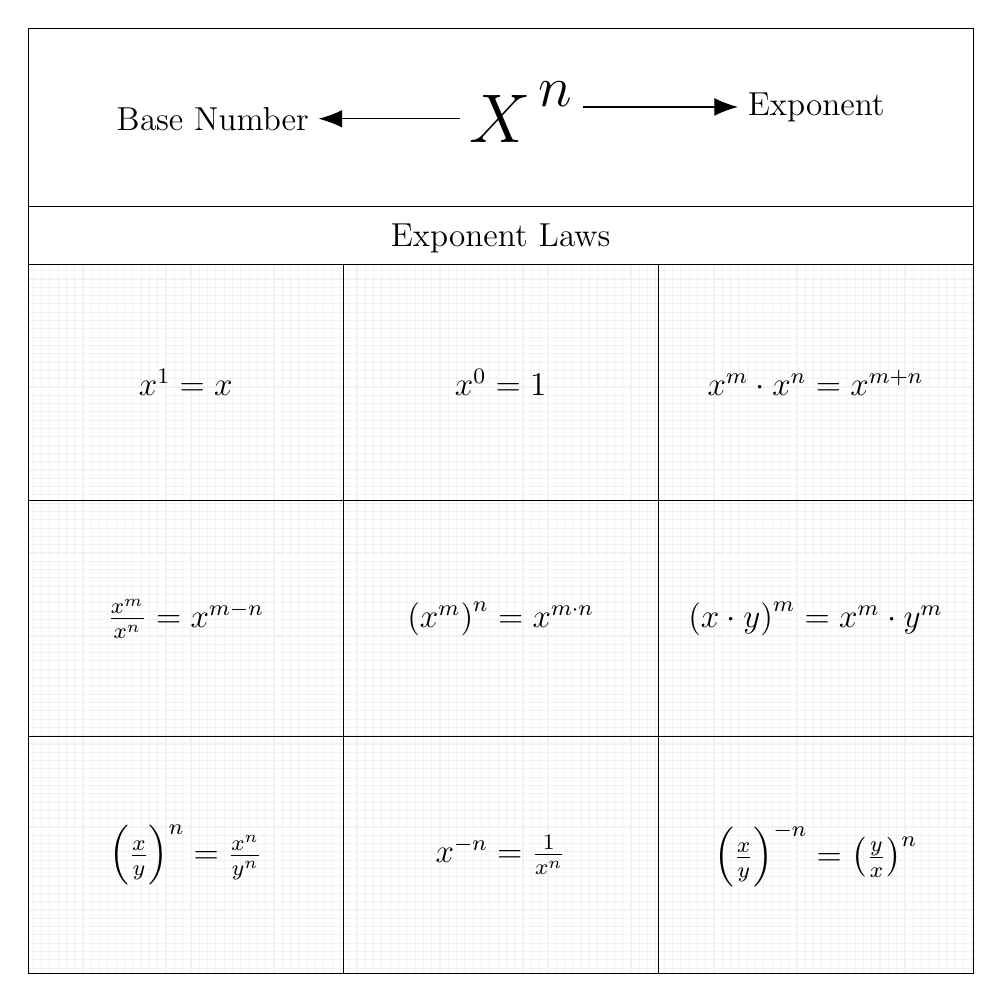
\begin{tikzpicture}[fill=white]
        \draw (0,0) rectangle (12,12);
        \draw[pattern=grid, pattern color=black!5] (0,0) rectangle (12,9);
        \draw (0,9.733) rectangle (12,9);

        % Exponent example.
        \draw (6.7,11) node (n) {\Huge{$^n$}}
            (11,11) node[anchor=east] (nn) {\large Exponent}
            (6,10.85) node (x) {\Huge{$X$}}
            (1,10.85) node[anchor=west] (xx) {\large Base Number}
            (6,9.33) node[anchor=center] (l) {\large Exponent Laws };
        \draw[-{Latex[length=3mm]}] (n) -- (nn);
        \draw[-{Latex[length=3mm]}] (x) -- (xx);

        % Grid guidelines.
        \draw[-, ystep=3, xstep=4] (0,0) grid (12,9);

        % Laws of exponents
        \draw[line width=5pt]
            (2,7.5) node[anchor=center] (x) {\large $x^1 = x$}
            (6,7.5) node[anchor=center] (x) {\large  $x^0 = 1$}
            (10,7.5) node[anchor=center] (x) {\large $x^m \cdot x^n = x^{m+n}$}

            (2,4.5) node[anchor=center] (x) {\large $\frac{x^m}{x^n} = x^{m - n}$}
            (6,4.5) node[anchor=center] (x) {\large $\left(x^m\right)^n = x^{m \cdot n}$}
            (10,4.5) node[anchor=center] (x) {\large $\left(x \cdot y\right)^m = x^m \cdot y^m$}

            (2,1.5) node[anchor=center] (x) {\large $\left(\frac{x}{y}\right)^n = \frac{x^n}{y^n}$}
            (6,1.5) node[anchor=center] (x) {\large $x^{-n} = \frac{1}{x^n}$}
            (10,1.5) node[anchor=center] (x) {\large $\left(\frac{x}{y}\right)^{-n} = \left(\frac{y}{x}\right)^n$};
    \end{tikzpicture}
}
\vspace{\fill}
\pagebreak

\subsection{Radicals}
\pagebreak

\section{Algebra}

\subsection{Expressions}
\vspace{\fill}
\begin{tikzpicture}[fill=white]
    \draw (-6,-6) rectangle (6,6);
        % Monomial
        % Binomial
        % Trinomial
        % Polynomial
        % Coefficient
        % Degrees
\end{tikzpicture}
\vspace{\fill}
\pagebreak

\subsection{Equations}
\vspace{\fill}
\begin{tikzpicture}[fill=white]
    \draw (-6,-6) rectangle (6,6);
        % Independent (in)
        % Dependent (out)
        % Balance
        % Linear
        %
        % Polynomial
        % Degrees
\end{tikzpicture}
\vspace{\fill}
\pagebreak

\subsection{Linear equations}
% They allow scientist to describe relationships between two variables in the
% physical world, make predictions, calculate rates, and make conversions.
\pagebreak

\subsection{Slopes}
% Slope intercept form
% Point slope form
\pagebreak

\subsection{Linear inequalities}
\pagebreak

\subsection{Systems of linear inequalities}
\pagebreak

\subsection{System of linear equations}
% When the lines intersect, the point of intersection is the only point that
% the two graphs have in common

% If the two lines are the same (on top of one another), there are infinite
% amounts of points in common.

% Elimination
% Sub
\pagebreak

\subsection{Quadratic equations}
\end{document}
